\documentclass[12pt,a4paper]{article}
\usepackage[utf8]{inputenc}
\usepackage[german]{babel}
\usepackage[T1]{fontenc}
\usepackage{amsmath}
\usepackage{amsfonts}
\usepackage{amssymb}
\usepackage{graphicx}
\usepackage{multicol}
\usepackage[left=2.5cm,right=2.5cm,top=2cm,bottom=2cm]{geometry}
\usepackage{float}
\author{Gruppe C14 \\ Julián Häck, Martin Koytek, Lars Wenning, Erik Zimmermann}
\begin{document}
\section{Bestimmung der Verdampfungsenthalpie von Wasser}
\subsection{Versuchsbeschreibung}
%Kurze Darstellung der physikalischen Grundlagen und Ziele der Versuche, %die zum Verständnis
%des Versuches/Protokolls benötigt werden. (max. 1 Seite)
Zur Bestimmung der Verdampfungsenthalpie wird die Verdampfungswärme in einem isochoren Prozess bestimmt, wodurch die Volumenarbeit verschwindet. Somit ist die Verdampfungsentalpie gleich der Verdampfungswärme. Grundlegend für den Versuch ist die Clausius-Clapeyronschen Gleichung:
\begin{equation}
\frac{dp}{dT}=\frac{\nu \Lambda}{T(V_1-V_2)}
\end{equation}
mit der Stoffmenge $\nu$, der Verdampfungswärme $\Lambda$ und der Differenz der Volumen(Gas,Flüssigkeit).
Unter der Annahme, dass das Gasvolumen von Wasserdampf deutlich größer (Faktor 1200) ist, als das Volumen von Wasser (flüssig), ergibt sich die DGL zu
\begin{equation*}
\frac{dp}{dT}=\frac{\nu \Lambda}{T\cdot V_{gas}}
\end{equation*}
Mit der Näherung des idealen Gases ($p\cdot V=\nu R T$) lässt sich die DGL lösen:
\begin{equation}
ln(\frac{p}{p_0})=-\frac{\Lambda}{R}(\frac{1}{T}-\frac{1}{T_0})
\end{equation}
bzw.
\begin{equation}
\ln(p)=-\frac{\Lambda}{R}\cdot \frac{1}{T}+c \text{ mit } c=const
\end{equation}
Nun wird der Druck und die Temperatur des Wasserdampfes beim Abkühlen gemessen und anschließend $\ln(p)$ gegen $\frac{1}{T}$ aufgetragen. Die Steigung ergibt sich dann zu $-\frac{\Lambda}{R}$ aus der dann die Verdampfungswärme $\Lambda$ bestimmt wird.
\subsection{Versuchsaufbau und Durchführung}
%Genaue Beschreibung der verwendeten Aufbauten unter Verwendung von %Skizzen oder Photos
%Beschreibung der Messwerterfassungseinstellungen (eingestellte %Messzeiten, Messbedingungen,
%5Trigger, Anzahl der Messungen) und der Durchführung der Versuche. (max. 1 Seite)
\begin{figure}[H]
\centering
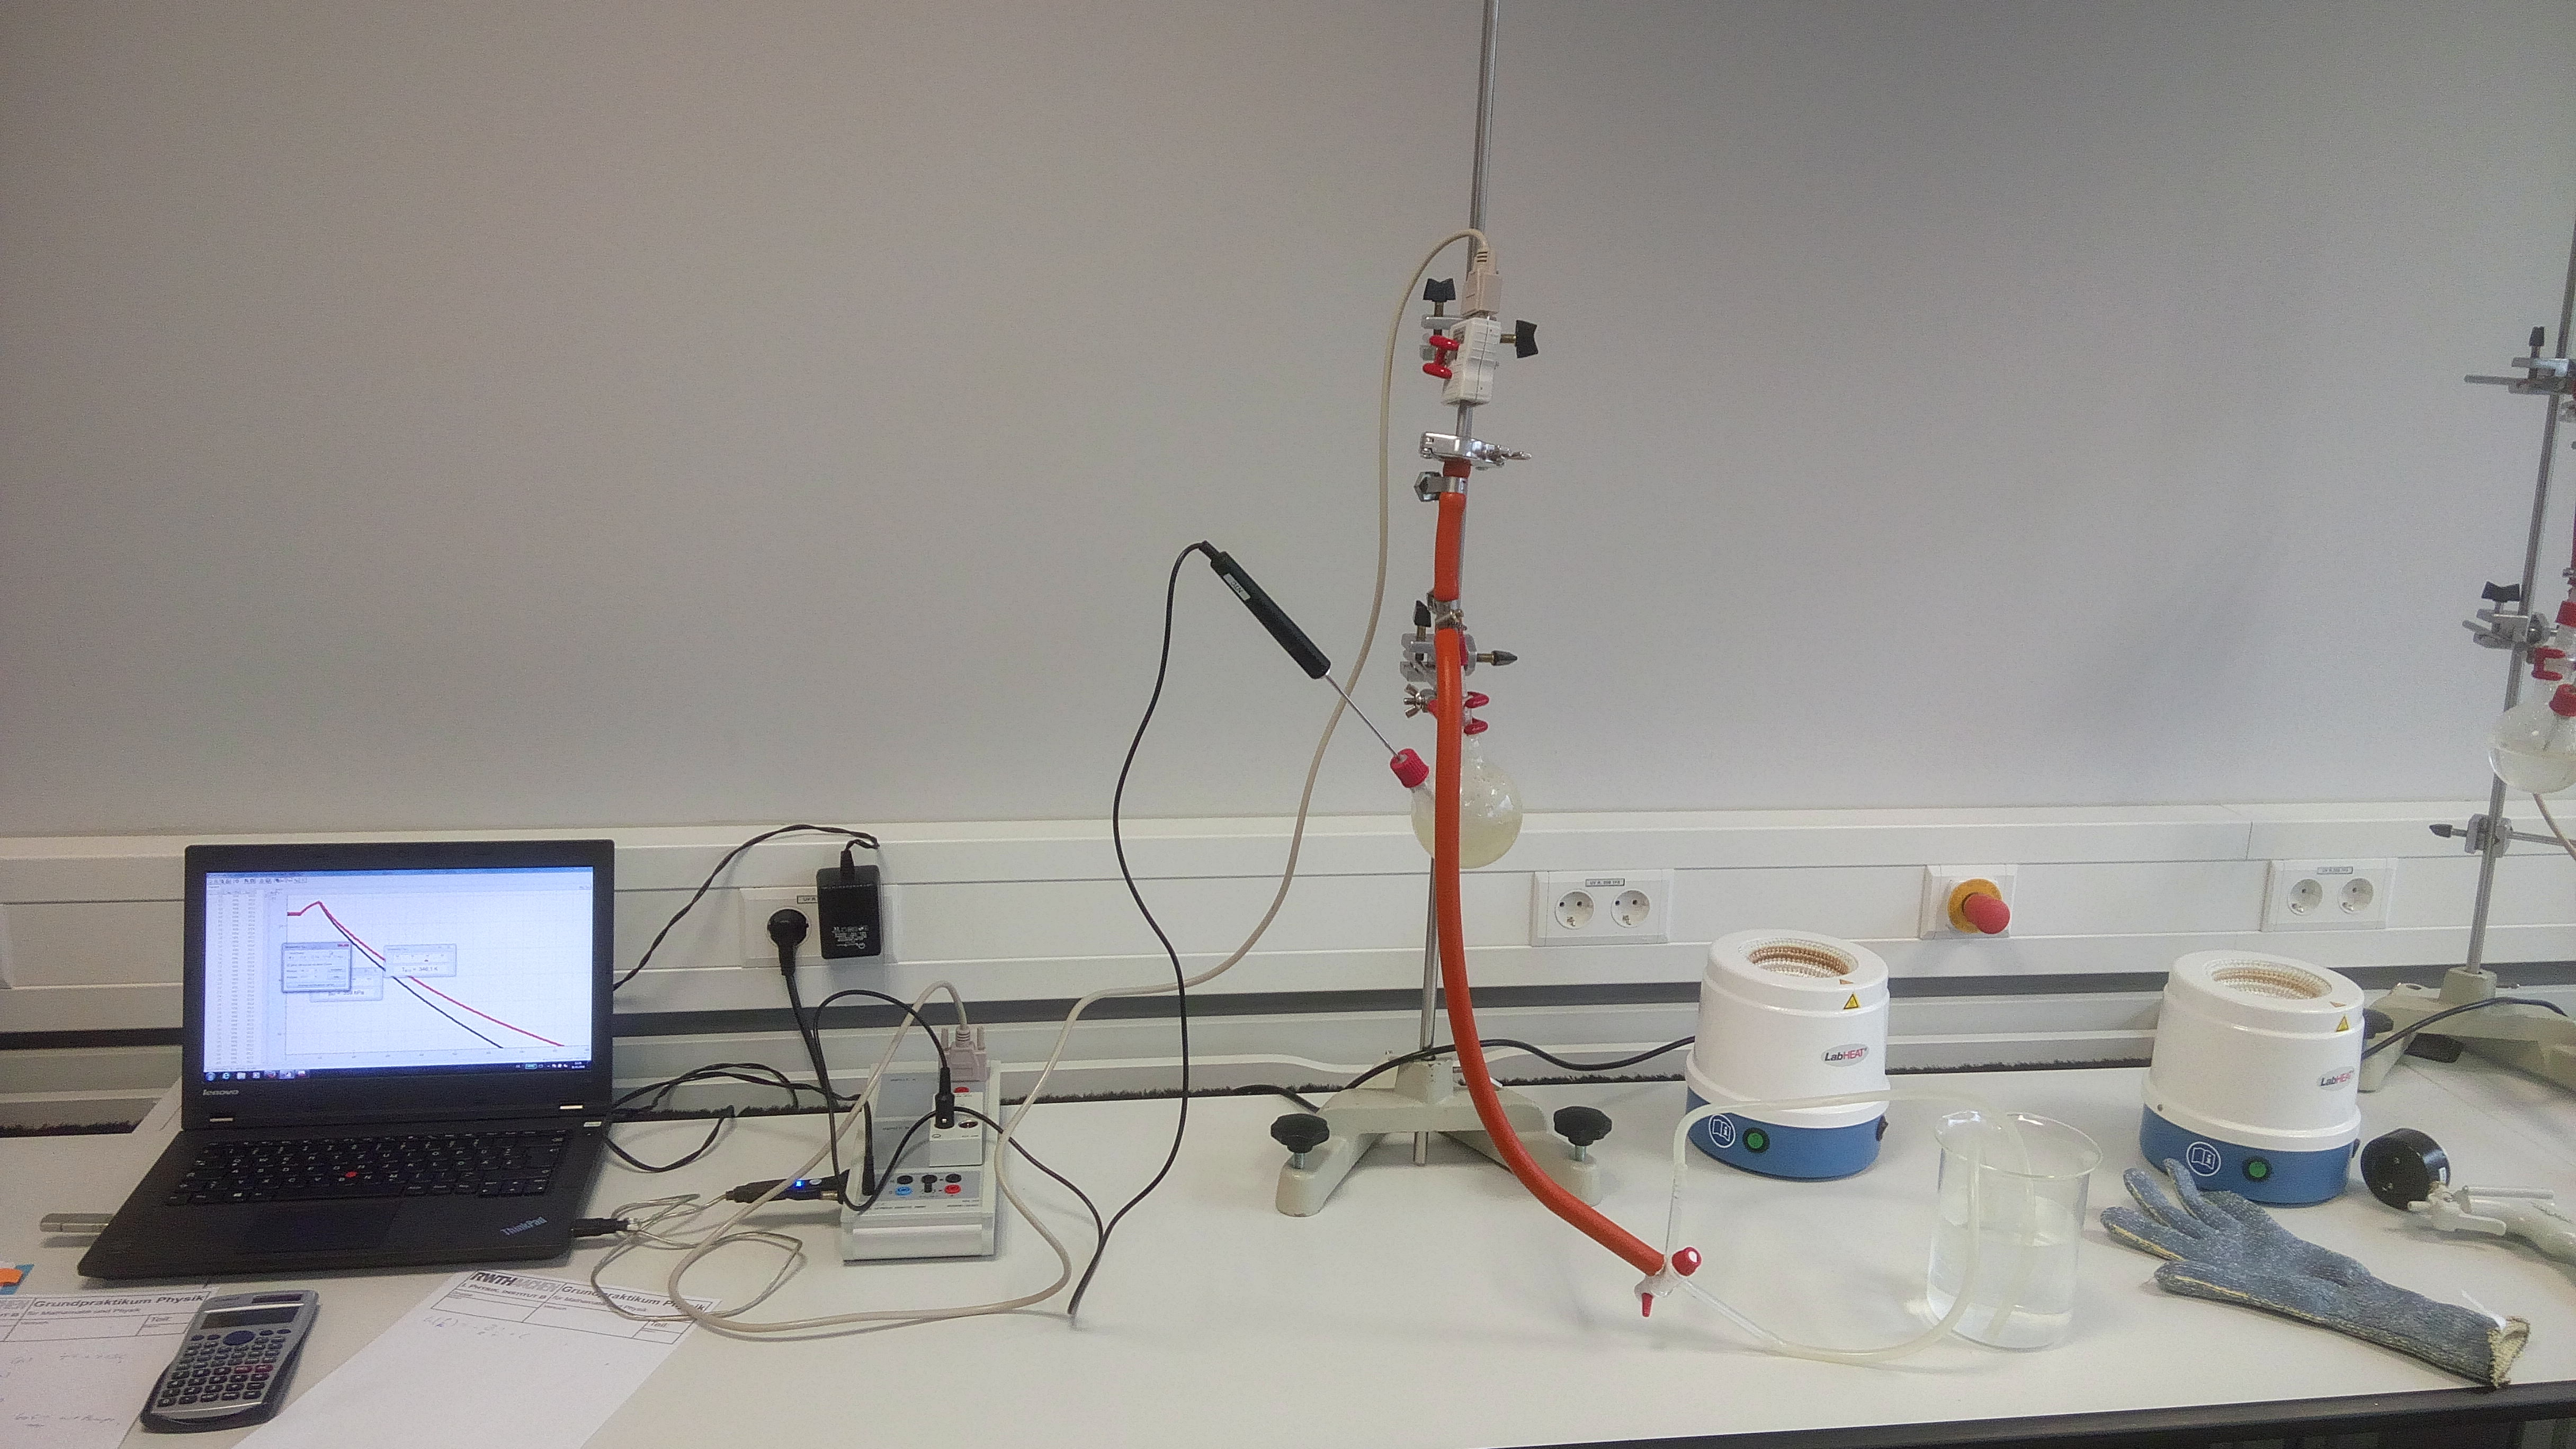
\includegraphics[scale=0.1]{Bilder/IMG_20160331_121650.jpg}
\caption{Versuchsaufbau während des Abkühlvorgangs}
\end{figure}
Benötigte Geräte:
\begin{multicols}{2}
\begin{itemize}
\item Sensor-Cassy
\item Heizhaube
\item Absolutdrucksensor mit Stativstange
\item Verbindungskabel
\item Temperatursensor
\item Temperaturbox
\columnbreak
\item Kolben
\item Messbecher
\item Glasventil
\item Stativ mit Stange
\item Schläuche
\item Verbindungsstücke
\item Muffen
\end{itemize}
\end{multicols}
\begin{table}[H]\centering \caption{Messparameter} \begin{tabular}{ccc} & Gruppe 1 & Gruppe 2 \\ \hline Intervall & 50ms & 100ms \\ Anzahl & 12000 & unbegrenzt \\ Messzeit & 600s & unbegrenzt \\ \end{tabular} \end{table}
Für diesen Versuch wurde der bereits mit Wasser befüllte Kolben nun mit Hilfe der Heizhaube erhitzt. Während des Erhitzens wurde das Ventil so gestellt, dass der Druck durch einen Schlauch in den Messbecher geleitet wurde, der vorher ebenfalls mit Wasser befüllt wurde. Dadurch wurde verhindert dass Luft zurück in den Kolben strömen konnte.
Nachdem die Siedetemperatur erreicht und möglichst viel Luft aus dem Kolben durch Wasserdampf verdrängt wurde, haben wir die Heizhaube entfernt, das Ventil geschlossen und die Messung gestartet.
\subsection{Versuchsauswertung}
\subsubsection{Rohdaten}
\begin{figure}[H]
\centering
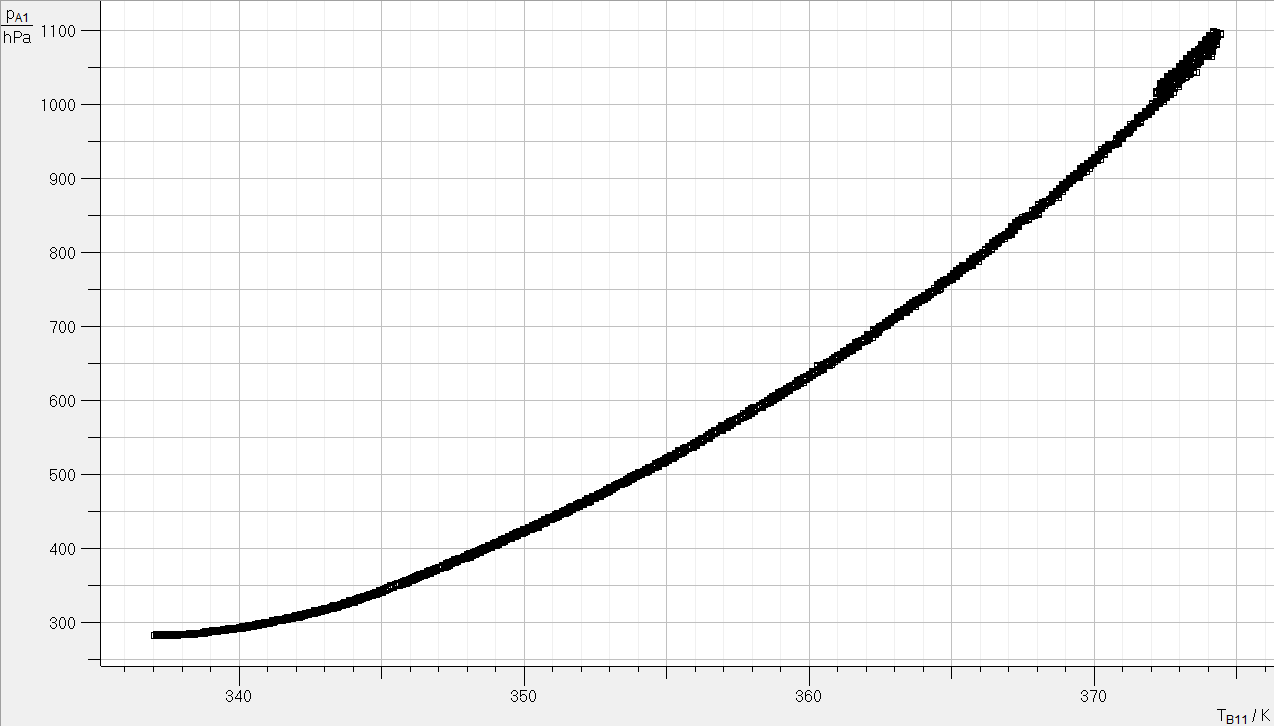
\includegraphics[scale=0.5]{Bilder/RohdatenHaupmessungGrp2.png}
\caption{Druck gegen Temperatur des Abkühlvorgangs Gruppe 2}
\end{figure}
\begin{figure}[H]
\centering
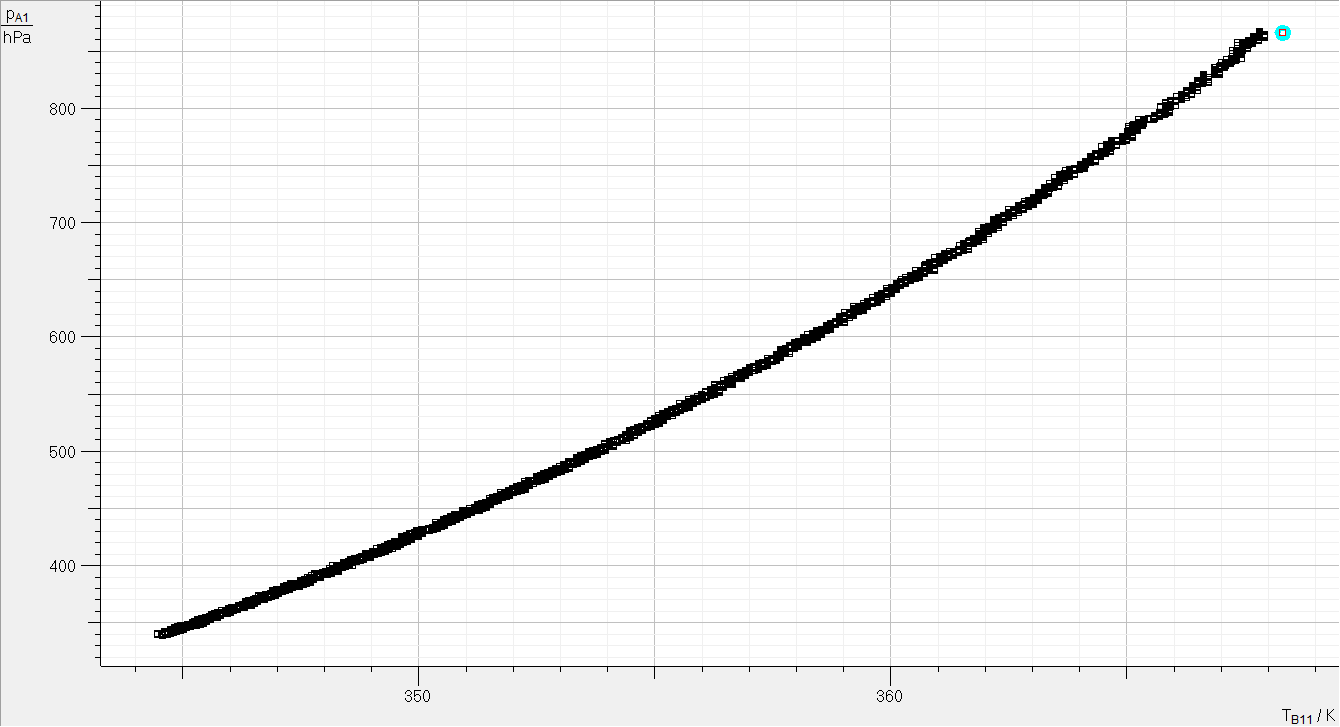
\includegraphics[scale=0.5]{Bilder/RohdatenHaupmessungGrp11.png}
\caption{Druck gegen Temperatur des Abkühlvorgangs Gruppe 1}
\end{figure}
\subsubsection{Transformation der Rohdaten/Analyse}
Zunächst wurden alle Werte unserer Messung umgeformt in $\ln(p)$ und $\frac{1}{T}$.
\begin{figure}[H]
\centering
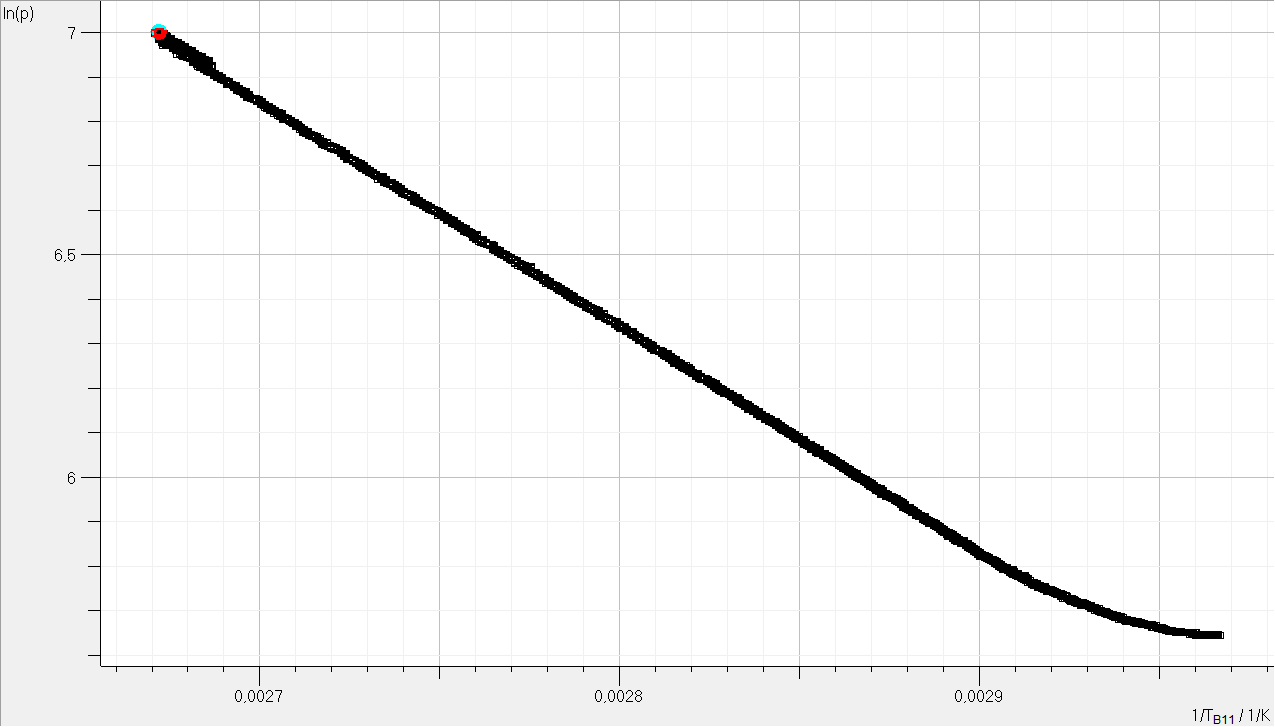
\includegraphics[scale=0.5]{Bilder/HauptmessungbearbeitetGrp2.png}
\caption{$\ln(p)$ gegen $\frac{1}{T}$ des Abkühlvorgangs Gruppe 2}
\end{figure}
Mit diesen Werten wurde anschließend eine Lineare Regression durchgeführt und durch die Werte mit ihren Fehlern geplottet. Dabei wurden die Werte in 16 Teile unterteilt um später die Temperaturabhängigkeit der Verdampfungswärme betrachten zu können.
\begin{figure}[H]
\centering
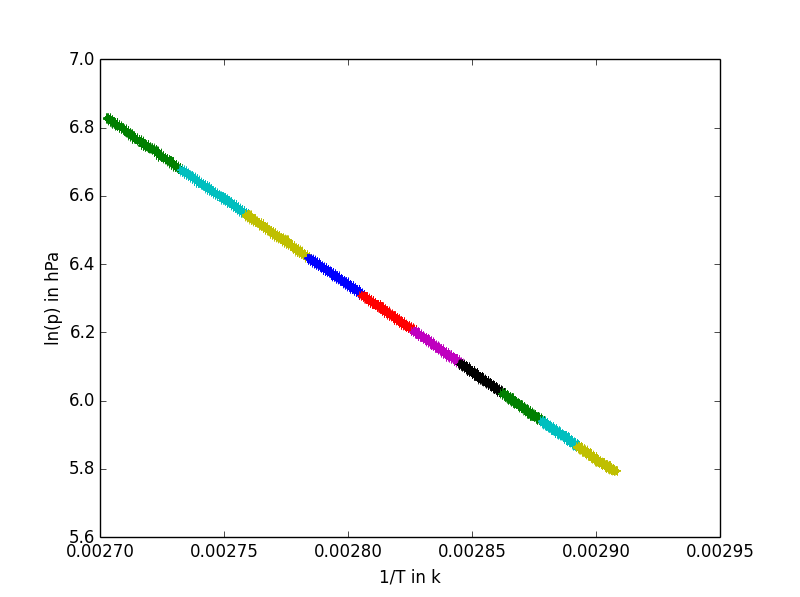
\includegraphics[scale=0.7]{Bilder/linreg_EL_neuerFehler.png}
\caption{Lineare Regression durch die umgeformten Messwerte, Randwerte wurden bereits entfernt Gruppe 2}
\end{figure}
\begin{figure}[H]
\centering
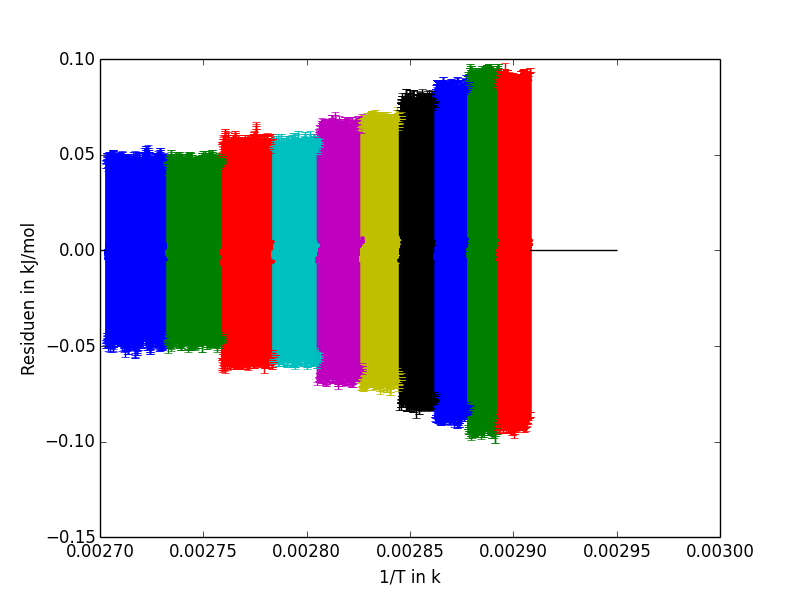
\includegraphics[scale=1]{Bilder/residuen_EL_neuerFehler.png}
\caption{Residuen zur Linearen Regression}
\end{figure}
\begin{figure}[H]
\centering
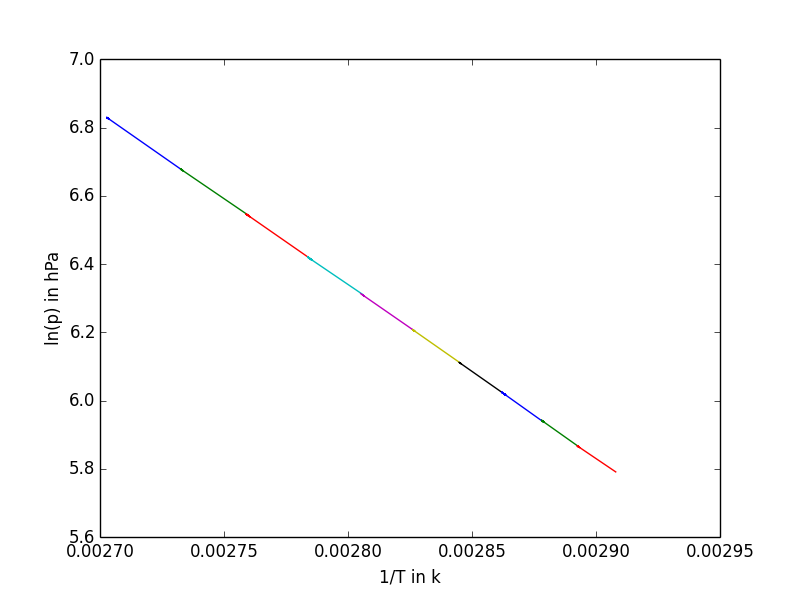
\includegraphics[scale=0.7]{Bilder/linreg_nurlinreg_EL.png}
\caption{Lineare Regression ohne Messwerte Gruppe 2}
\end{figure}
\begin{itemize}
\item $\frac{\chi^2}{f} \Rightarrow 1.27 | 0.96 | 1.12 | 0.86 | 0.89 | 0.77 | 0.79 | 0.78 | 0.71 | 0.74$
\end{itemize}
Die Steigung der Linearen Regression ergibt sich zu $-\frac{\Lambda}{R}$, sodass sich daraus nun unser Ergebnis für $\Lambda$ berechnen lässt.
\begin{table}[H]\centering
\caption{Ergebnisse Gruppe 1}

\begin{tabular}{c|c|c|c|c}
Abschnitt&T in K&$\Lambda$ in $\frac{kJ}{mol}$&$\sigma_{\Lambda_{stat}}$in $\frac{kJ}{mol}$&$\sigma_{\Lambda_{sys}}$in $\frac{kJ}{mol}$\\
\hline
1&366.37&41.74&0.342&0.513\\
2&363.81&42.08&0.327&0.519\\
3&361.65&43.27&0.339&0.534\\
4&359.72&41.62&0.324&0.515\\
5&358.0&42.51&0.327&0.526\\
6&356.39&43.34&0.294&0.537\\
7&354.95&42.88&0.272&0.532\\
8&353.53&42.65&0.365&0.53\\
9&352.27&41.19&0.327&0.513\\
10&351.06&44.01&0.384&0.547\\
11&349.95&41.45&0.395&0.517\\
12&348.87&41.2&0.299&0.514\\
13&347.84&42.88&0.406&0.535\\
14&346.86&45.11&0.432&0.563\\
15&345.91&39.82&0.446&0.499\\
16&344.99&40.41&0.414&0.506\\
17&343.32&41.56&0.143&0.521\\
18&342.4&38.78&0.163&0.488\\
19&341.57&42.03&0.212&0.528\\
20&340.68&36.24&0.175&0.458\\
21&339.78&37.06&0.189&0.468\\
\end{tabular}
\end{table}

\begin{table}[H]\centering
\caption{Ergebnisse Gruppe 2}
\begin{tabular}{c|c|c|c|c}
Abschnitt&T in K&$\Lambda$ in $\frac{kJ}{mol}$&$\sigma_{\Lambda_{stat}}$in $\frac{kJ}{mol}$&$\sigma_{\Lambda_{sys}}$in $\frac{kJ}{mol}$\\
\hline
1&367.93&42.18&0.273&0.518\\
2&364.13&41.17&0.156&0.508\\
3&360.76&41.96&0.102&0.518\\
4&357.71&40.97&0.1&0.508\\
5&355.03&41.8&0.12&0.519\\
6&352.6&42.24&0.117&0.525\\
7&350.38&42.31&0.136&0.527\\
8&348.4&43.03&0.141&0.537\\
9&346.54&42.79&0.162&0.535\\
10&344.83&40.84&0.175&0.512\\
\end{tabular}
\end{table}
Anschließend wurden die Ergebnisse für $\Lambda$ gegen die Temperatur aufgetragen.
\begin{figure}[H]
\centering
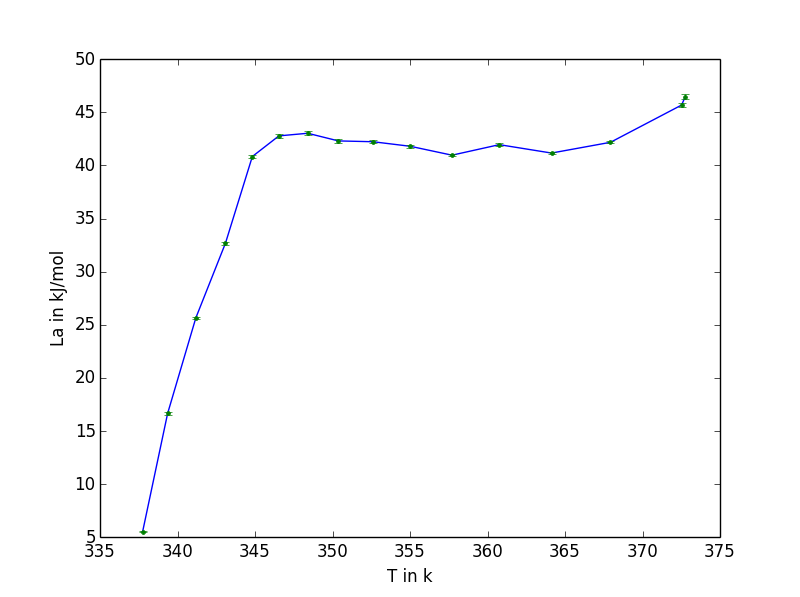
\includegraphics[scale=0.7]{Bilder/lamda_EL_neuerFehler.png}
\caption{Verdampfungswärme gegen Temperatur Gruppe 2}
\end{figure}
Die ersten vier so wie die letzten zwei Werte wurden in allen anderen Plots ausgelassen. Hier sieht man, dass dies sinnvoll war, da diese noch während des Aufheizens bzw. nachdem das Wasser nicht mehr siedete aufgezeichnet wurden. 
\subsubsection{Fazit}
Allgemein lässt sich sagen, dass der Versuch in beiden Gruppen sehr gut abgelaufen ist. Das Abdichten hat gut geklappt und das Aufheizen sowie das Vermessen der Daten beim Abkühlen hat keine Probleme gemacht.
Die Anpassung unserer Linearen Regressionen durch die Messwerte waren nach den $\frac{\chi^2}{f}$ zu urteilen, sinnvoll.
Die errechneten Werte für $\Lambda$ liegen alle in der gleichen Größenordnung wie der im Skript angegebene Literaturwert von $40.6 \frac{kJ}{mol}$.
Wenn man die Werte mit der Tabelle(\ref{lambdaskirpt}) vergleicht, liegen die Abweichungen zwischen 1 und 10 $\sigma$. 
Die Auftragung von $\Lambda$ gegen $T$ liefert leider kein sinnvolles Ergebnis, was wohl an den Näherungen in den benutzten Gleichungen liegt.
Beispiele dafür sind: Ideale Gasgleichung, Vernachlässigen des Wasservolumens und das Vernachlässigen der Volumenänderung beim Erhitzen bzw. Abkühlen.

\section{Anhang}
\begin{figure}[H]
\centering
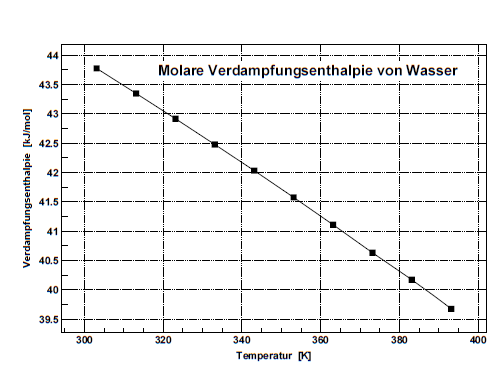
\includegraphics[scale=0.7]{Bilder/Verdampfungsentalpie.PNG}
\label{lambdaskirpt}
\caption{Verdampfungsentalpie gegen Temperatur aus dem Skript}
\end{figure}
\begin{figure}[H]
\centering
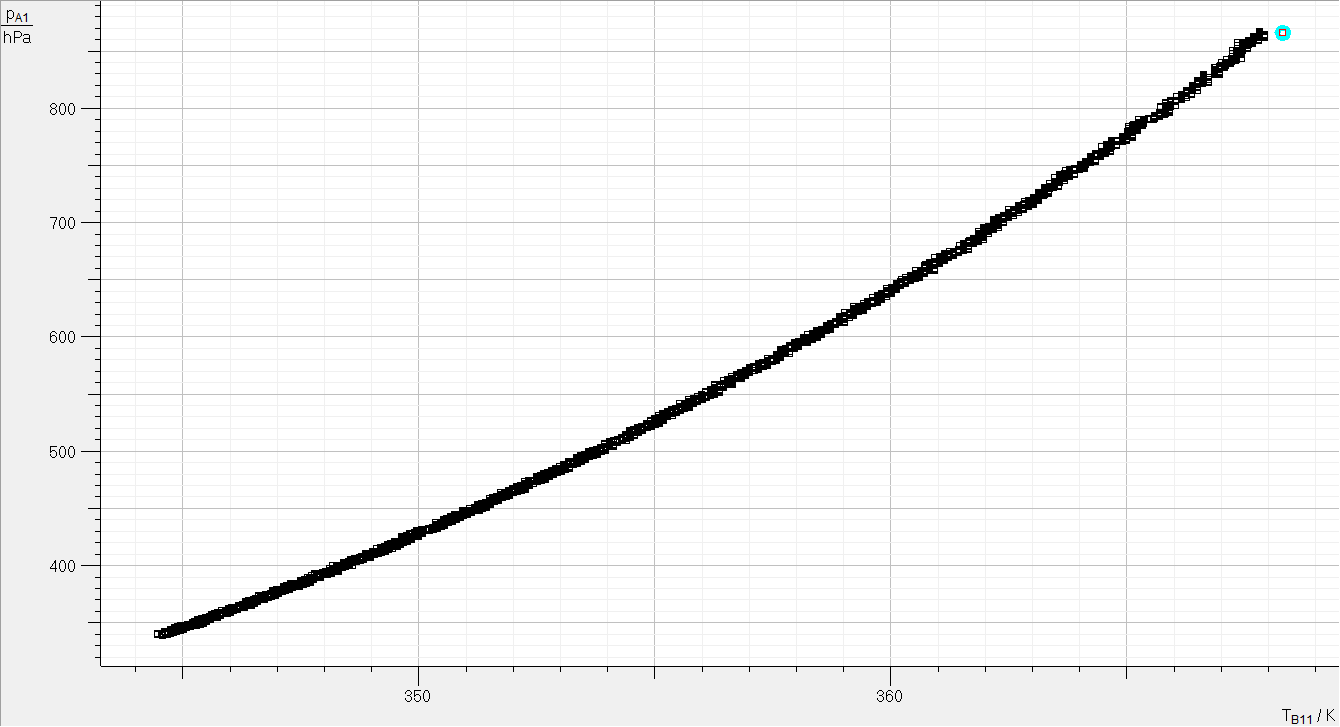
\includegraphics[scale=0.5]{Bilder/RohdatenHaupmessungGrp11.png}
\caption{1. Rohdaten Gruppe 1}
\end{figure}
\begin{figure}[H]
\centering
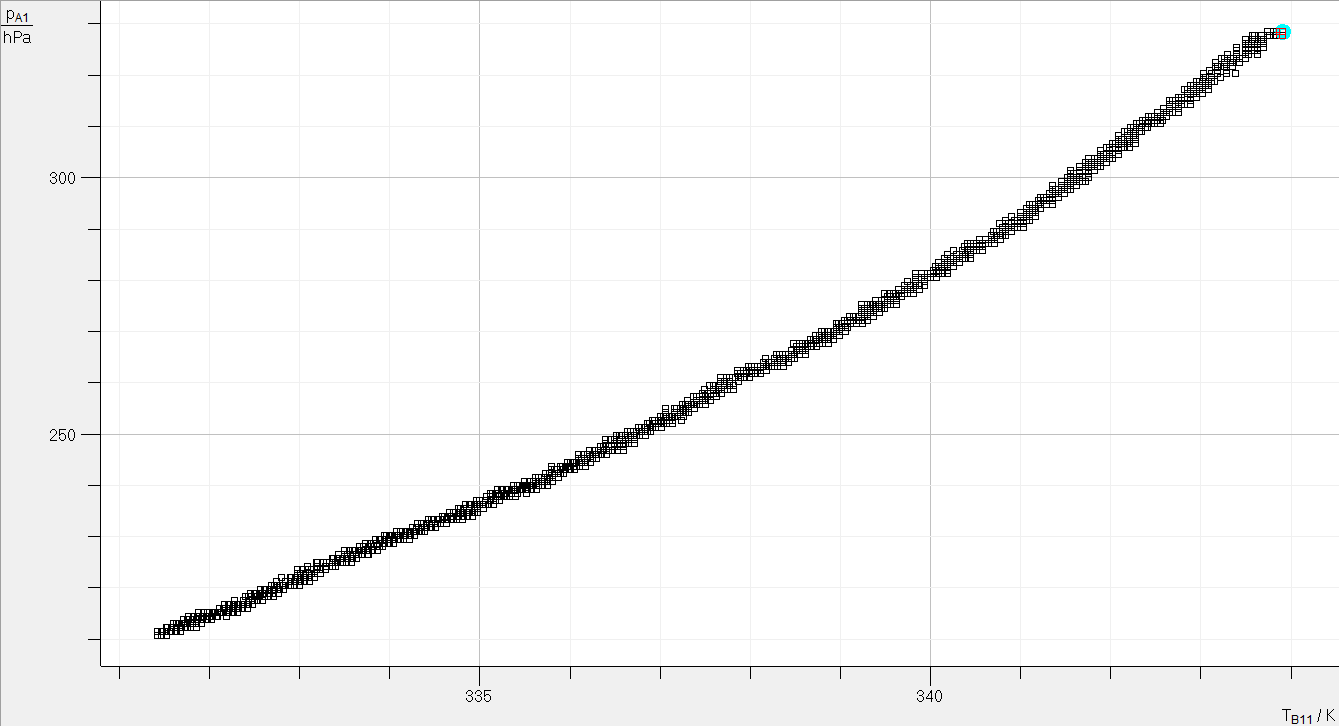
\includegraphics[scale=0.5]{Bilder/RohdatenHaupmessungGrp12.png}
\caption{2. Rohdaten Gruppe 1}
\end{figure}
\begin{figure}[H]
\centering
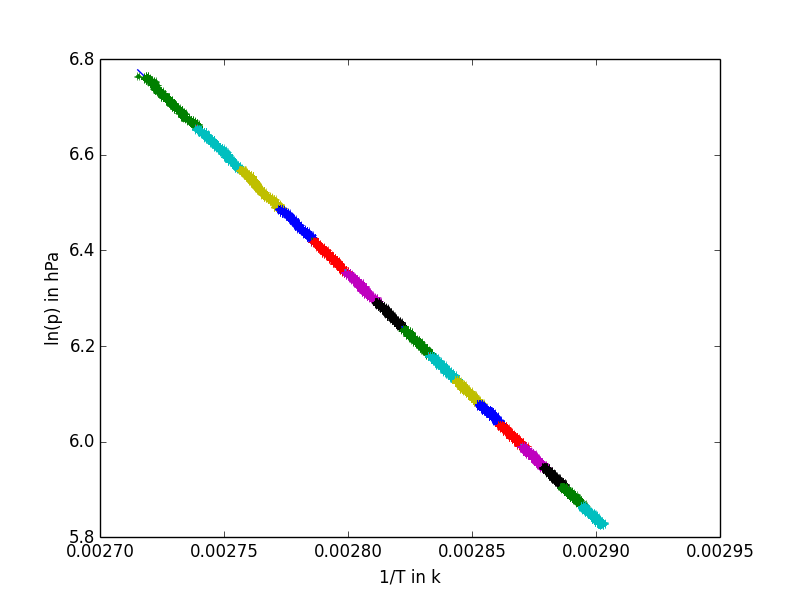
\includegraphics[scale=0.7]{Bilder/linreg_lambda_JM_1.png}
\caption{1. Lineare Regression Hauptmessung Gruppe 1}
\end{figure}
\begin{figure}[H]
\centering
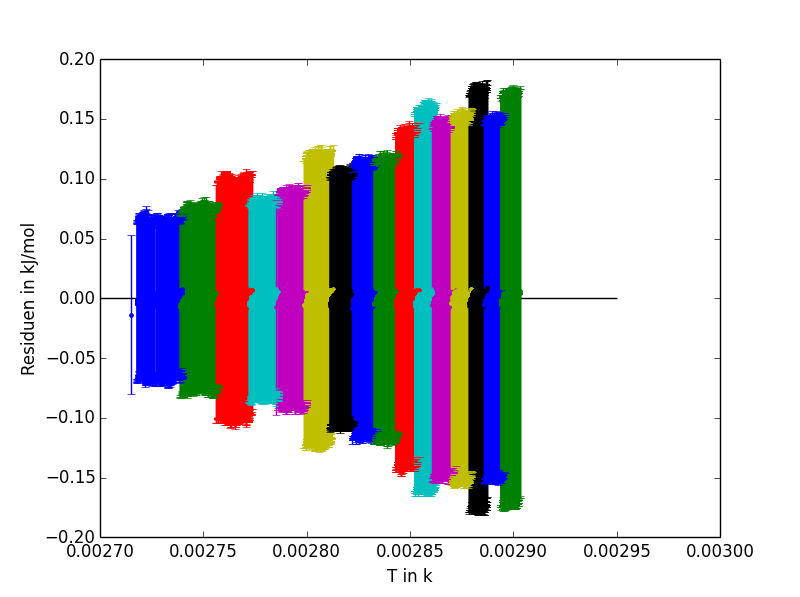
\includegraphics[scale=0.7]{Bilder/residuen_JM_1.png}
\caption{Residuen zur 1. Linearen Regression Hauptmessung Gruppe 1}
\end{figure}
\begin{figure}[H]
\centering
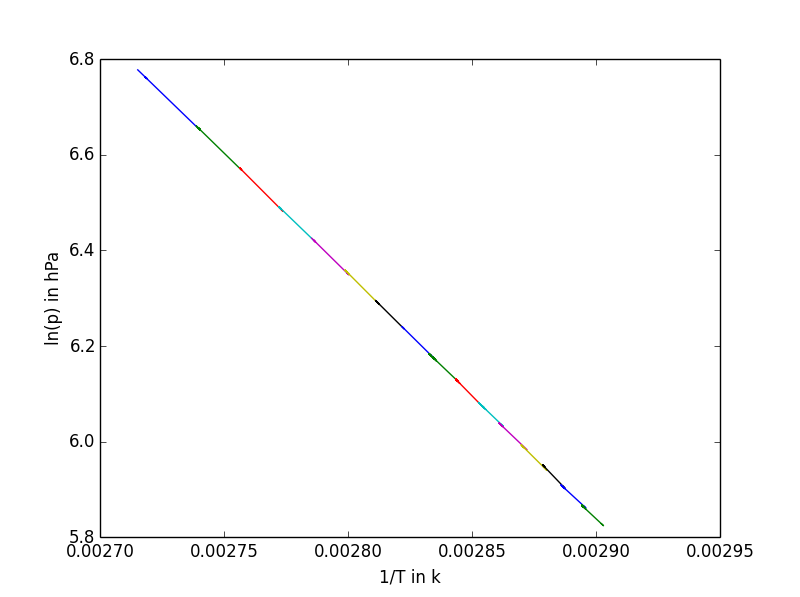
\includegraphics[scale=0.7]{Bilder/linreg_nurlinreg_JM_1.png}
\caption{1. Lineare Regression Hauptmessung Gruppe 1 ohne Messwerte}
\end{figure}
\begin{figure}[H]
\centering
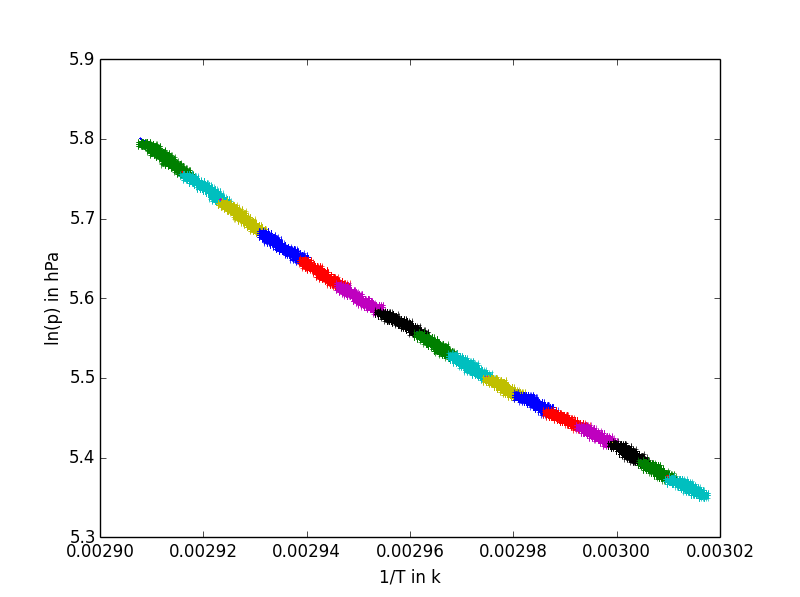
\includegraphics[scale=0.7]{Bilder/linreg_lambda_JM_2.png}
\caption{2. Lineare Regression Hauptmessung Gruppe 1}
\end{figure}
\begin{figure}[H]
\centering
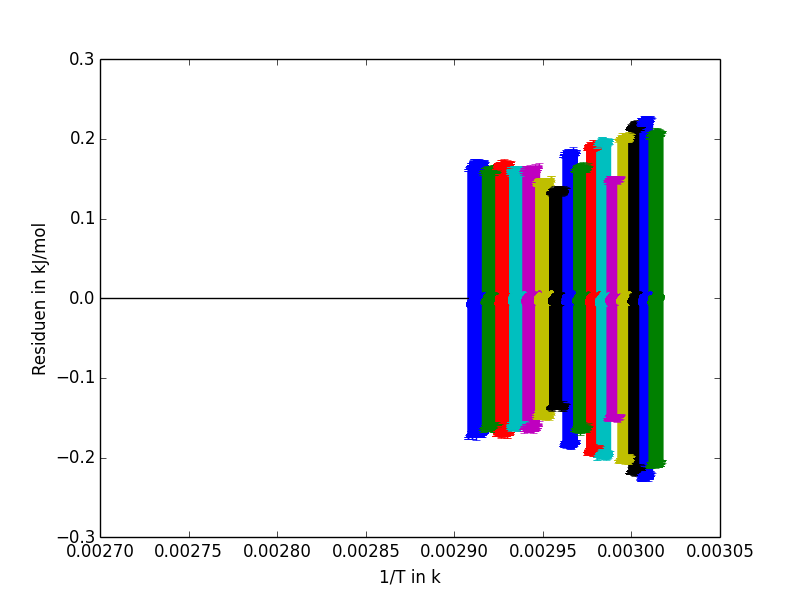
\includegraphics[scale=0.7]{Bilder/residuen_JM_2.png}
\caption{Residuen zur 2. Lineare Regression Hauptmessung Gruppe 1}
\end{figure}
\begin{figure}[H]
\centering
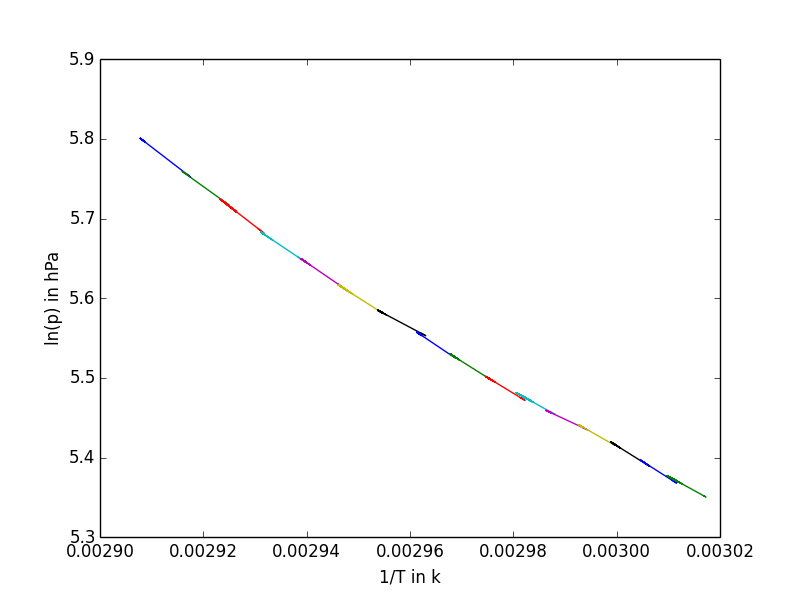
\includegraphics[scale=0.7]{Bilder/linreg_nurlinreg_JM_2.png}
\caption{2. Lineare Regression Hauptmessung Gruppe 1 ohne Messwerte}
\end{figure}
\begin{figure}[H]
\centering
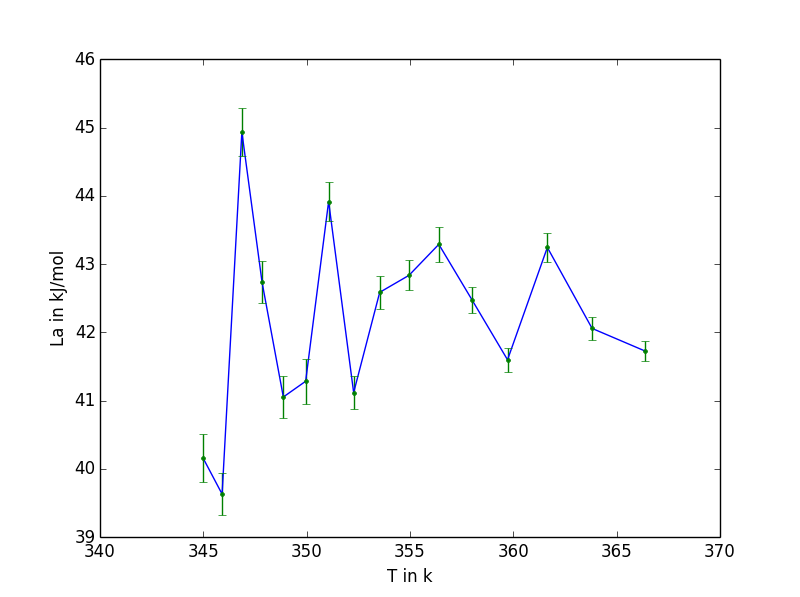
\includegraphics[scale=0.7]{Bilder/lamda_JM_1.png}
\caption{1. $\Lambda$ gegen $T$ Gruppe 1}
\end{figure}
\begin{figure}[H]
\centering
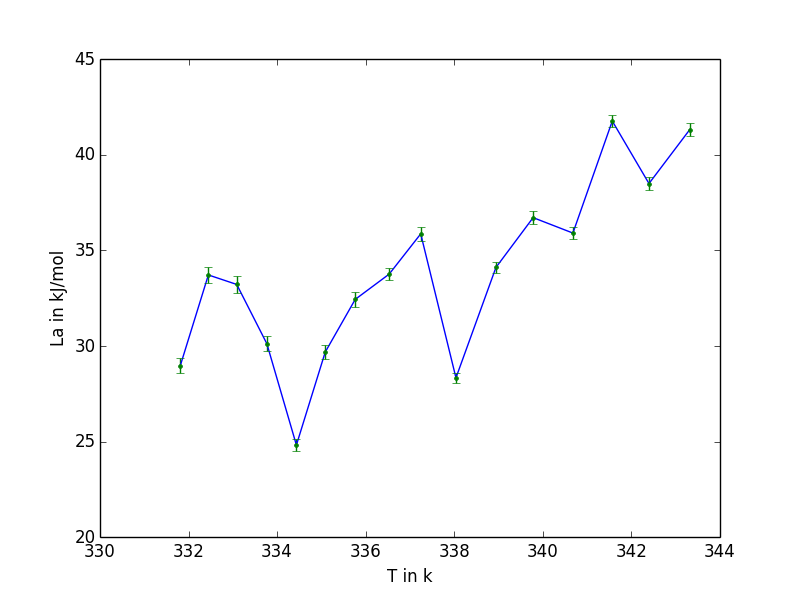
\includegraphics[scale=0.7]{Bilder/lamda_JM_2.png}
\caption{2. $\Lambda$ gegen $T$ Gruppe 1}
\end{figure}

\end{document}